\chapter{Patrones de software aplicados a la seguridad}

\section{Proxy Pattern}

El \textbf{patrón Proxy} es un patrón de diseño estructural que proporciona un \textbf{objeto sustituto o intermediario} para controlar el acceso a otro objeto. Este patrón se utiliza cuando, por alguna razón, no es conveniente o posible interactuar directamente con el objeto real, ya sea por cuestiones de control de acceso, optimización de rendimiento, o administración de recursos.

\begin{figure}[H]
    \centering
        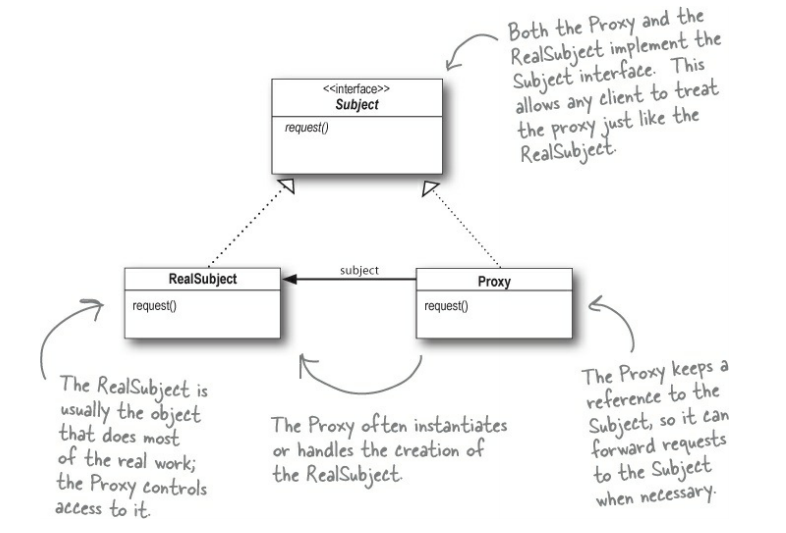
\includegraphics[width=0.5\linewidth]{PatronesSoftware/proxypattern.png}
        \caption{Proxy Pattern}
        \label{fig:proxy-pattern}
\end{figure}

\textbf{Analogía:} Una tarjeta de crédito es un \textbf{proxy} para una cuenta bancaria, la cual es un \textbf{proxy} para un conjunto de dinero en efectivo. Ambas implementan la misma interfaz: pueden usarse para realizar un pago. El consumidor se siente bien porque no necesita llevar grandes cantidades de efectivo. El dueño de la tienda también está contento, ya que el ingreso de una transacción se agrega electrónicamente a la cuenta bancaria de la tienda sin el riesgo de perder el depósito o ser robado en el camino al banco. 

El \textbf{patrón Proxy} puede utilizarse para controlar el acceso a un recurso o servicio, y para realizar autenticación, autorización, registro de actividades (logging) o almacenamiento en caché. Esto puede prevenir accesos no autorizados y ataques de \textbf{inyección SQL}.


\section{Facade Pattern}

El \textbf{patrón Facade} puede utilizarse para proporcionar una interfaz simplificada a un sistema o subsistema complejo, ocultando sus detalles internos y complejidad. Esto puede reducir el acoplamiento y el riesgo de exponer información o funcionalidades sensibles. Puede mejorar la \textbf{modularidad} y \textbf{mantenibilidad} de tu código al separar el subsistema en capas o componentes, así como proteger el subsistema de accesos no autorizados o maliciosos mediante la implementación de verificaciones de seguridad y políticas en la fachada. 

\begin{figure}[H]
    \centering
    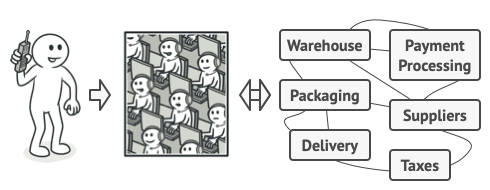
\includegraphics[width=0.5\linewidth]{PatronesSoftware/facade.png}
    \caption{Facade Pattern}
    \label{fig:facade-pattern}
\end{figure}

\textbf{Analogía:} Cuando llamas a una tienda para hacer un pedido por teléfono, un operador actúa como tu \textbf{fachada} ante todos los servicios y departamentos de la tienda. El operador te proporciona una interfaz de voz simple para el sistema de pedidos, las pasarelas de pago y varios servicios de entrega. 

\textbf{Para implementar el patrón Facade}, primero se debe identificar el subsistema que deseas simplificar y asegurar, analizar sus clases, métodos, dependencias e interfaces. Luego, crear una\textbf{ clase fachada }que proporcione una interfaz simple y unificada para el subsistema, con métodos que correspondan a las funcionalidades que los clientes necesitan. Los métodos de la fachada también deben realizar cualquier verificación de seguridad o validación antes de acceder al subsistema. Finalmente, refactoriza los clientes para que utilicen la clase fachada en lugar de interactuar directamente con el subsistema; los clientes solo deben comunicarse con la fachada.

\section{Adapter Pattern}

El \textbf{patrón Adapter} (Adaptador) es un patrón de diseño estructural que permite que dos interfaces incompatibles trabajen juntas. Funciona como un traductor entre dos clases, convirtiendo la interfaz de una clase en otra que el cliente espera, sin cambiar el código existente. Esto podría mejorar la \textbf{interoperabilidad} y \textbf{compatibilidad} de los componentes de tu software, así como prevenir errores o inconsistencias. 

\textbf{Analogía: }Cuando viajas de los EE.UU. a Europa por primera vez, puede que te lleves una sorpresa al intentar cargar tu computadora portátil. Los estándares de los enchufes y tomas de corriente son diferentes en los distintos países. Por eso, tu enchufe de EE.UU. no encajará en una toma de corriente alemana. El problema se puede resolver usando un adaptador de enchufe que tenga el enchufe de estilo americano y la clavija de estilo europeo.

\begin{figure}[H]
    \centering
    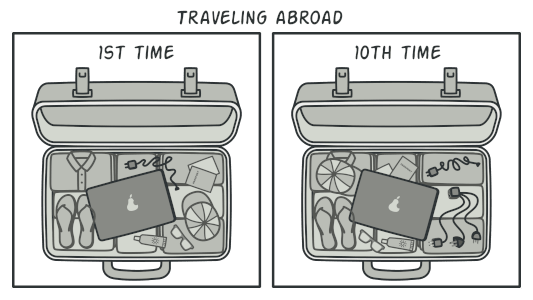
\includegraphics[width=0.5\linewidth]{PatronesSoftware/adapter.png}
    \caption{Adapter Pattern}
    \label{fig:adapter-pattern}
\end{figure}

\textbf{Ejemplo:} Podría usarse un adaptador para traducir las consultas SQL de la aplicación moderna en consultas compatibles con la base de datos antigua, mientras que también implementas medidas de seguridad como parametrización de consultas o escape de caracteres para prevenir SQL Injection. El adaptador actúa como una capa de seguridad entre la base de datos vulnerable y la aplicación moderna, proporcionando una mayor protección sin necesidad de migrar completamente la base de datos.

\section{Singleton}

\textbf{Singleton} es un patrón de diseño creacional que te permite garantizar que una clase tenga solo una instancia, mientras proporciona un punto de acceso global a esta instancia. Puede ayudar a controlar el acceso a recursos sensibles, evitando que partes no autorizadas interfieran con componentes críticos. Ayuda a centralizar las configuraciones relacionadas con la seguridad, asegurando una aplicación consistente de las mismas. 

\begin{figure}[H]
    \centering
    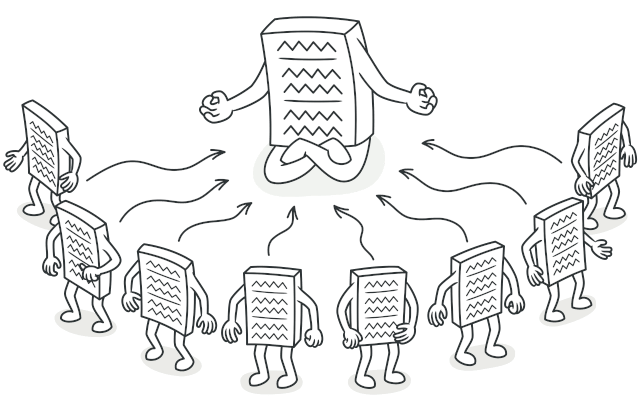
\includegraphics[width=0.5\linewidth]{PatronesSoftware/singleton.png}
    \caption{Singleton Pattern}
    \label{fig:singleton-pattern}
\end{figure}


\textbf{Analogía: }El gobierno es un excelente ejemplo del patrón Singleton. Un país solo puede tener un gobierno oficial. Independientemente de las identidades personales de las personas que forman los gobiernos, el título 'El Gobierno de X' es un punto de acceso global que identifica al grupo de personas a cargo.

El patrón \textbf{Singleton} puede ser útil cuando se necesita controlar el acceso y el comportamiento de un recurso compartido, como una conexión a la base de datos, un archivo de configuración o un registrador (logger). Uno de los beneficios del patrón Singleton es que puede mejorar la seguridad del sistema al garantizar la consistencia y prevenir el acceso no autorizado o la modificación del recurso compartido. 

Por ejemplo, si se utiliza una clase Singleton para gestionar una conexión a la base de datos, puedes asegurarte de que solo los usuarios autorizados puedan acceder a la base de datos y realizar las operaciones permitidas. También se puede implementar verificaciones de seguridad y mecanismos de registro (logging) en la clase Singleton para monitorear y auditar las actividades en la base de datos. El patrón Singleton también puede prevenir problemas de concurrencia y corrupción de datos al sincronizar el acceso al recurso compartido.


\section{Observer}

El patrón \textbf{Observer} es un patrón de diseño de comportamiento que permite definir un mecanismo de suscripción para notificar a múltiples suscriptores sobre cualquier evento que ocurra en el objeto que están observando. 

\textbf{Analogía: }Si te suscribes a un periódico o revista, ya no necesitas ir a la tienda para ver si el próximo número está disponible. En su lugar, el editor envía los nuevos números directamente a tu buzón tan pronto como se publica, o incluso con antelación. El editor mantiene una lista de suscriptores y sabe a qué revistas están interesados. Los suscriptores pueden salir de la lista en cualquier momento si desean que el editor deje de enviarles los nuevos números de la revista.

\begin{figure}[H]
    \centering
    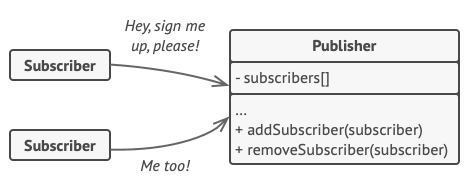
\includegraphics[width=0.5\linewidth]{PatronesSoftware/observer.png}
    \caption{Observer Pattern}
    \label{fig:observer-pattern}
\end{figure}

\textbf{Monitoreo de seguridad en tiempo real:} Imagina que tienes diferentes componentes de seguridad en una red o aplicación, como un sistema de detección de intrusiones (IDS), un firewall, o un antivirus. Usando el patrón \textbf{Observer}, estos sistemas pueden observar eventos importantes que ocurren en el sistema, como accesos no autorizados, intentos de inyección de \ACRshort{sql} o actividad sospechosa. Cuando el sistema principal detecta un evento de seguridad, notifica a todos los observadores (componentes de seguridad) para que tomen las acciones correspondientes (como bloquear una IP, generar una alerta o iniciar un análisis). 

\textbf{Notificación de eventos de seguridad:} En una aplicación o servidor web, podrías tener múltiples observadores que estén pendientes de eventos de seguridad, como la creación de nuevas cuentas de usuario o el acceso a archivos sensibles. Cada vez que ocurre un evento, los observadores pueden recibir una notificación y actuar en consecuencia (alertar a los administradores, registrar la actividad, activar un sistema de defensa, etc.).

\textbf{Autenticación y control de acceso: }En un sistema de control de acceso, podrías tener observadores que vigilan eventos como inicios de sesión fallidos o accesos a recursos sensibles. Si un observador detecta un patrón sospechoso (como demasiados intentos fallidos), puede notificar a otros componentes del sistema para bloquear la cuenta o iniciar un proceso de autenticación más fuerte.

\section{Decorator}

El patrón \textbf{Decorator} es un patrón de diseño estructural que te permite agregar nuevos comportamientos a los objetos colocando estos objetos dentro de objetos envolventes especiales que contienen los comportamientos. A diferencia de la herencia, que altera el comportamiento de un objeto de manera estática, el patrón Decorator ofrece flexibilidad para añadir o quitar comportamientos sobre la marcha sin necesidad de modificar la clase original.

\begin{figure}[H]
    \centering
    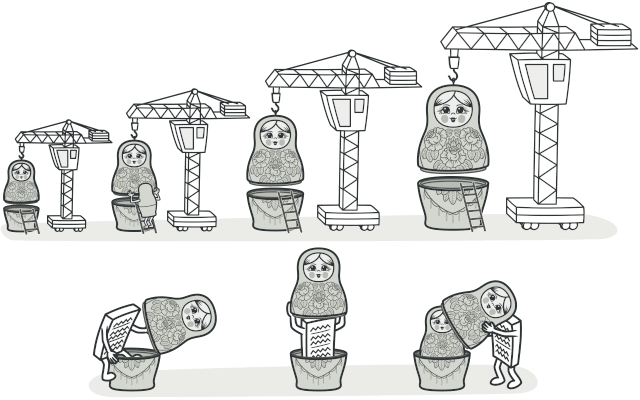
\includegraphics[width=0.5\linewidth]{PatronesSoftware/decorator.png}
    \caption{Decorator Pattern}
    \label{fig:decorator-pattern}
\end{figure}
Analogía: Imagina que tienes un objeto que representa un \textbf{mensaje} en una aplicación. Inicialmente, el mensaje solo tiene la funcionalidad de mostrar texto. Si deseas añadirle características como \textbf{cifrado}, \textbf{compresión}, o \textbf{registro de auditoría} de manera dinámica, puedes envolver el objeto \textbf{mensaje} en varios decoradores que proporcionen estas funcionalidades adicionales sin cambiar la clase original del mensaje. 

El patrón \textbf{Decorator} se puede emplear para agregar capas de seguridad a los objetos de manera dinámica, lo que permite implementar características como \textbf{validación de entradas} y \textbf{codificación de salidas}. Permite la \textbf{adición dinámica de características de seguridad}, adaptándose a las amenazas que evolucionan constantemente.

\section{Strategy}

El patrón \textbf{Strategy} es un patrón de diseño de comportamiento que te permite definir una familia de algoritmos, poner cada uno de ellos en una clase separada y hacer que sus objetos sean intercambiables. Este patrón es útil cuando deseas cambiar el comportamiento de un sistema en tiempo de ejecución, sin modificar el código que usa ese comportamiento.

El patrón \textbf{Strategy} es ideal para \textbf{adaptar algoritmos de seguridad} en función de diferentes tipos de ataques o requisitos de seguridad. Al usar este patrón, puedes implementar múltiples estrategias de seguridad (como cifrado, autenticación, validación, etc.) y elegir cuál usar dependiendo de la situación, sin cambiar la lógica principal del sistema.

\begin{figure}[H]
    \centering
    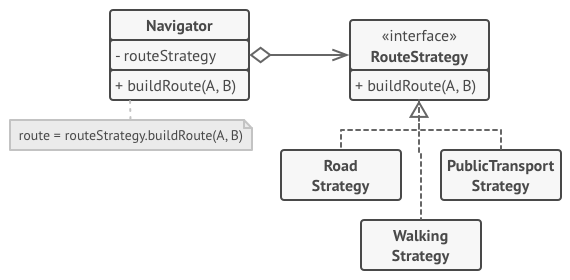
\includegraphics[width=0.5\linewidth]{PatronesSoftware/strategy.png}
    \caption{Strategy Pattern}
    \label{fig:strategy-pattern}
\end{figure}

\textbf{Patrones de diseño y su contribución a la seguridad del software} 

Los patrones de diseño pueden mejorar la seguridad del software al promover el uso de soluciones arquitectónicas probadas y buenas prácticas que mitigan vulnerabilidades comunes. Algunos beneficios clave que los patrones de diseño pueden ofrecer en este ámbito:

\subsubsection{1. \textbf{Encapsulamiento de datos sensibles}}

Los patrones de diseño ayudan a encapsular los datos sensibles, reduciendo el riesgo de vulnerabilidades derivadas de componentes no protegidos o datos inseguros. Patrones como el \textbf{Proxy} permiten acceder a componentes sensibles de manera controlada, previniendo accesos no autorizados.

\subsubsection{2. \textbf{Manejo y prevención de errores}}

Los patrones de diseño también mejoran el manejo de errores y excepciones, evitando que estos se propaguen por la aplicación. Un manejo adecuado de errores es clave para evitar que las vulnerabilidades sean explotadas.

\subsubsection{3. \textbf{Reusabilidad del código}}

Al fomentar la reutilización del código, los patrones de diseño permiten que los desarrolladores utilicen soluciones probadas y seguras, lo que incrementa la robustez del software. El uso de patrones evita la duplicación de código y hace más fácil la aplicación de soluciones de seguridad ya validadas.

\subsubsection{4. \textbf{Mantenibilidad y adaptabilidad}}

Los patrones de diseño promueven la creación de código modular y extensible, facilitando su modificación o extensión sin introducir nuevos riesgos de seguridad. Esto también hace más fácil realizar mejoras o ajustes en la arquitectura de seguridad conforme emergen nuevas amenazas.

\subsubsection{5. \textbf{Pruebas y depuración}}

Al estructurar el código de manera más organizada y modular, los patrones de diseño facilitan las pruebas y la depuración, lo que permite identificar y corregir vulnerabilidades antes de que lleguen a producción. Un código más estructurado es más fácil de probar y asegurar.

\subsubsection{Ventajas generales de los patrones de diseño en seguridad}

Al adherirse a estos patrones de diseño, los desarrolladores establecen una base sólida para las prácticas de codificación segura. Estos patrones no solo ayudan a gestionar la seguridad de manera eficiente, sino que también promueven la mantenibilidad, escalabilidad y resistencia frente a los desafíos de seguridad emergentes.

Sin embargo, Un patrón no es necesariamente una \textbf{mejor práctica} para todos los dominios de problemas o lenguajes, por lo que es importante tratarlos como un conjunto de herramientas, en lugar de soluciones preempaquetadas. Dicho esto, hay \textbf{principios básicos de seguridad} que son esenciales. En particular, nunca confiar en la entrada externa. Siempre se debe sanear los datos de entrada del usuario, realizar validaciones sobre los datos externos, utilizar las características del lenguaje para escapar o parametrizar valores, y escribir pruebas para resultados inválidos al realizar conversiones explícitas de datos en el código.